\documentclass{article}

\usepackage{amsmath, amssymb}
\usepackage{graphicx}


\title{Rapport de projet IMA201}
\author{Jules Lefèvre, Manel Wafra} 
\date{28/11/2024}

\begin{document}

\maketitle
\begin{abstract}
    Nous présentons notre implémentation de la méthode ACoPa, qui consiste à extraire de chaque image une palette de couleur automatique, à des fins de compression ou stylistiques. On associera pour cela l'alogirthme des K-moyennes à une étude de la couleur de l'image, à l'aide d'un traîtement des histogrammes de la saturation, la teinte et l'intensité. Ce traîtement se fera en implémentant une méthode novatrice de segmentation d'histogramme. On comparera enfin les résultats expérimentaux de notre algorithme aux algorithme plus traditionnels comme K-means ou Median cut.
\end{abstract}
\section{Introduction}
\subsection{Définition du problème}
Le cerveau humain est capable de traiter des images avec peu de couleurs en se basant sur les contrastes globaux de l'image, et en extrapolant sur la couleur moyenne d'un objet. Ainsi, ce qui fait qu'on reconnaît une cocinelle sur une feuille, ce n'est pas le degradé des couleurs de la coccinelle mais bien le contraste entre le rouge, les points noirs, et le vert de la feuille. 
    \begin{figure}[h]
        \begin{subfigure}{0.5\textwidth}
            \centering
            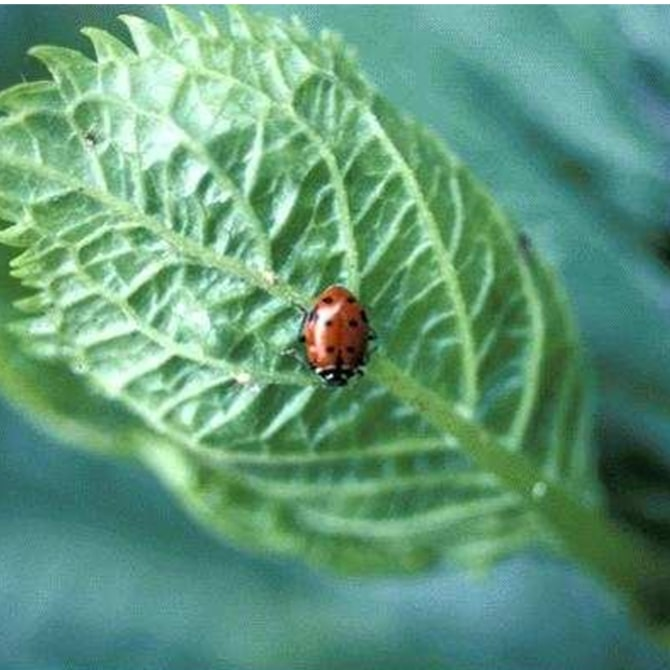
\includegraphics{./images_test/cocci_petit.jpg}
            \caption{Coccinelle sur une feuille}
            \label{fig :image1}
        \end{subfigure}
        \begin{subfigure}{0.5\textwidth}
            \centering
            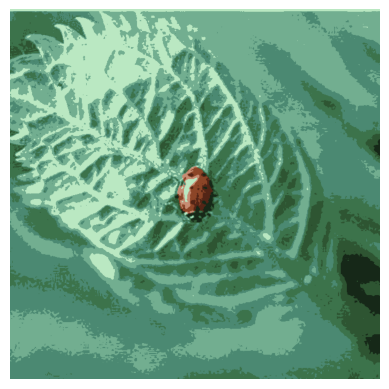
\includegraphics{./test_projets/cocci_petit_acopa.png}
            \caption{La même image compressée}
            \label{fig :image2}
        \end{subfigure}
        \caption{Comparaison entre une image originale et une image compressée}
        \label{fig: side by side}
    \end{figure}
Ainsi, réduire le nombre de couleur dans une image ne représente pas une perte massive d'informations, à priori bien sûr de conserver certaines propriétés comme la rareté des couleurs (coccinelle rouge sur une majorité de vert.)

La question se pose cependant du nombre de couleurs à conserver. Est il possible de savoir à l'avance combien de couleurs garder pour chaque image en minimisant la perte d'informations, et encore mieux d'automatiser le problème ? 

Les deux problèmes qu'on vient d'évoquer ne sont pas anodins, puisqu'ils sont ceux qu'on a très vite rencontré en essayant d'implémenter les méthodes traditionelles de classification sur l'espace des couleurs d'une image, que nous allons maintenant aborder.
\subsection{Méthodes traditionelles : K-means}
K-means est une méthode d'apprentissage non-supervisée utilisé pour le partitionnage de donées.\\

\noindent {\itshape \textbf{Algorithme :}} \\
Soit $(k_n)_{n \in \mathbb{N}} \in K^n$ avec $k_i \neq k_j \ \forall (i,j), \ i \neq j$. \\
On procède comme suit :
\begin{enumerate}
    \item Initialisation : $\forall i \leq n, \ C_i = \{k_i\}$.
    \item Pour chaque point $k \in K$, faire :
    \begin{enumerate}
        \item Calculer $p = \arg\min_{i \in [0;n]} D(k, k_i)$, où $D$ est une distance définie.
        \item Mettre à jour $C_p = C_p \cup \{k\}$.
    \end{enumerate}
    \item Pour tout $i \in [0;n]$, recalculer : $k_i = \text{mean}(C_i)$.
\end{enumerate}

En itérant ce procédé un certain nombre de fois, on obtient une classification des points de l'ensemble initial.

\bigskip

{\itshape \textbf{Limites de K-Means :}} \\
Le nombre de centroïdes (et donc de classes finales) ainsi que le nombre d'itérations sont arbitraires :
\begin{itemize}
    \item On peut fixer le nombre d'itérations en définissant un critère de convergence, par exemple lorsque la distance entre les centroïdes actuels et précédents devient inférieure à un seuil donné.
    \item Cependant, le nombre de classes finales (le nombre de centroïdes $k$) ne peut pas être prédéfini sans un pré-traitement des données. Cela constitue une limitation bien connue de l'algorithme K-Means.
\end{itemize}

De plus, l'initialisation aléatoire des centroïdes peut conduire à des classifications incohérentes.

\bigskip

{\itshape \textbf{Application à des données RGB :}} \\
On peut appliquer l'algorithme K-Means à un problème lié aux couleurs en définissant une distance dans l'espace RGB comme suit :
\[
D(k, k_i) = \| k - k_i \|^2 = \sum_{\text{canaux RGB}} (k - k_i)^2.
\]
Cette norme au carré calcule la différence canal par canal, et sert de métrique pour regrouper les couleurs de manière significative. \\

On obtient donc des palettes de couleur, comme attendu. Cependant, on ne respecte aucune des deux conditions. Le nombre de couleur est arbitraire, et on ne minimise donc pas forcément le nombre de couleur. On ne minimise pas non plus la perte d'information, puisque on peut perdre l'informations des couleures dites rares. Par exemple, en appliquant notre k-moyenne à l'image de la coccinelle, on obtient : 

On a donc perdu l'information de la couleur rouge de la coccinelle, et donc une bonne partie de l'information de l'image.

\subsection{Méthodes traditionelles : Median Cut}
Median cut est un algorithme de tri qui permet de sélectionner récursivement des représentants d'une palette de couleur.

 \noindent{{\itshape \textbf{Algorithme :}} }
\begin{enumerate}
    \item Initialisation : l = [] \\ $\forall i \in I, \ l = \ l \cup\{i\} $.
    \item Iteration : Calculer le canal RGB qui a la plus grande variance selon la liste l. Prendre la médiane de ce canal et séparer les points en deux listes $l_1$ et $l_2$, en fonction de leur position par rapport à la médiane selon le canal. Itérer avec $l_1$ et $l_2$. 
    \item On arrête d'itérer quand on a le bon nombre de classe. On définit la valeur de chaque pixel d'une classe sur la valeur du pixel moyen.
    \end{enumerate}
    \item .
\bigskip
\end{enumerate}

\noindent{{\itshape \textbf{Limites de Median-cut :}}} \\
On retrouve les mêmes problèmes que dans K-Moyennes. On ne peut pas automatiser le nombre de classes renvoyés par Median-cut, donc on ne minimise pas forcément le nombre de couleurs ou la perte d'information. 
\section{Prétraitement des données}
\subsection{Contexte}
Comme nous l'avons vu à traver les exemples de K-moyennes et median cut, les algorithmes de classification traditionelles ne sont pas cabales de minimiser le nombre de couleurs tout en gardant le maximum d'informations. Il nous faut donc trouver un moyen de quantifier ces information et de les extraire de l'image. Une première idée est de passer dans l'espace HSI, qui est plus riche en information propre à la classification couleur que l'espace RGB. En particulier, la teinte est porteuse d'informations sur la rareté des couleurs, car une couleur rare et donc précieuse se démarquera sur l'histogramme des teintes. Il nous faut donc trouver un moyen de repérer les couleurs sur ce dit histogramme, à l'aide d'un algorithme de segmentation. Or, on remarque que la présence d'une couleur en quantité suffisante dans une image se traduit souvent par une distribution à peu près unimodal autour de la valeur de teinte centrale de la couleur. L'objectif va donc être de détecter ces phases unimodales. Une fois qu'on a discriminé les couleurs principales de l'image, on va chercher à discriminer les couleurs entre elle en utilisant la saturation. On va répéter le processus ci-dessus, pour repérer les distributions significatives autour d'une valeur de saturation. Enfin, on répète ce processus sur la saturation. 
\subsection{Phases unimodales}
Il nous faut définir de manière plus rigoureuse les phases unimodales. 
Pour une histogramme h , on commence par définir l'estimateur de grenander de h comme le meilleur estimateur décroissant ou croissant de l'histogramme. 
On l'obtient en appliquant l'algorithme des Pool Adjacent Violators : \\
\noindent {\itshape \textbf{Algorithme :} \\
On définit l'opérateur $D : P(L) \rightarrow P(L) $ définit par : \\ 
\begin{itemize}
    \item Pour \( r = (r_i)_{i=1,\dots,n} \in P(L) \) et pour chaque intervalle \([i,j]\) sur lequel \(r\) est croissant :
    \[
    D(r)_k = \frac{r_i + \dots + r_j}{j-i+1} \quad \forall k \in [i,j].
    \]
    
    \item \( D(r)_k = r_k \) sinon.
\end{itemize}
En appliquant D à l'histogramme un nombre fini de fois, inférieur à la taille de ce dernier on obtient l'estimateur de Grenander décroissant de h : $\Bar{h}$
On peut de même définir l'estimateur de Grenander croissant d'un histogramme.\\

\textbf{Définition 1} : On dit qu'un histogramme h suit l'hypothèse de croissance (décroissance) sur un intervalle I si pour un test statistique T, on a que $h_{|I}$ est une réalisation de la loi définie par $\Bar{h_{|I}}$\\

Maintenant qu'on a définit les hypotèses de croissance et décroissance, la définition de l'unimodalité vient naturellement. \\

\textbf{Définition 2} : On dit qu'un histogramme h est unimodal sur un segment [a,b] si il existe $c \in [a,b]$ tq h suit l'hypothèse de croissance sur [a,c] et h suit l'hypothèse de décroissance sur [c,b] .

Il nous reste cependant à explorer la question du test statistique T dont il est question dans l'hypothèse de croissance.

\subsection{ Tests statistiques }
Dans le papier automatic color palette, il est question d'un test statistique T pour évaluer si un histogramme est bien la réalisation d'un test T.
Les chercheurs font référence à Kolomogorov-Smirnov ou au Chi-2, en disant que ces test fonctionnent. Cependant, ils ont eux même implémenté un test statistique qui permet de vérifier l'hypothèse. 

C'est ce test que nous avons d'abord essayé d'implémenter. 
\subsubsection{Test du NFA}
Soit h = $ (hi)_{i=1,...,L}$ un histogramme tel que $\sum_{i=1}^{L}h_i = N.$
Pour tout segment [a,b] de \{1,...,L\}, 
r(a,b) = $\frac{1}{N}(\sum_{i=a}^{b}h_i) $ la proportion des points dans [a,b]\\
Soit p = $(p_i)_{i=1,...,L}$ un probabilité discrète qu'on suppose être la loi de h. \\
Pour tout segment [a,b] de \{1,...,L\}, soit p(a,b) la probabilité qu'un point tombe dans [a,b] : \\
p(a,b) = $\sum_{i=1}^{L}p_i $
Pour tester l'hypothèse $H_0$ que p est la loi de h, on peut donc comparer pour tous les [a,b] les similarités entre r(a,b) et p(a,b). 
Sous $H_0$ la proba que [a,b] contienne au moins Nr(a,b) points parmis N est donnée par B(N,Nr(a,b),p(a,b)) avec : \\
B(n,j,p) = $\sum_{i=j}^{n} \binom{n}{i}p^i(1-p)^{n-i}$ \\
On a aussi que la proba que [a,b] contienne moins de r(a,b) éléments est donnée par B(N,N(1-r(a,b)),1-p(a,b))\\
\textbf{Définition 1} :\\
On definit pour chaque [a,b] le nombre de fausse alarme : \\

$NFA_{p}([a,b]) = \begin{cases}
\frac{L(L+1)}{2}B(N,Nr(a,b),p(a,b)) & \text{si} \ r(a,b) \geq p(a,b) \\
\frac{L(L+1)}{2}B(N,N(1-r(a,b)),1-p(a,b)) & \text{sinon}
\end{cases}
$
\textbf{Définition 2} : \\
On dit donc qu'un intervalle [a,b] est un rejet $\epsilon-significatif$ de $H_0$ si : \\ 
$NFA_p([a,b]) \leq \frac{\epsilon}{2}$\\
\textbf{Proposition 1: } \\
Sous l'hypothèse $H_0$, l'espérance du nombre de segment [a,b] qui sont des rejets $\epsilon-significatifs$ est inférieure à $\epsilon$ \\
\textbf{Proposition 2: } \\
On dit qu'un histogramme h suit la loi p sur [1,L] si h ne contient aucun rejet significatif de $H_0$\\
\textbf{Définition 3} : Soit r = $\frac{1}{N}h$ et $\Bar{r}$ l'estimateur de grenander de r. [a,b] est un rejet significatif de l'hypothèse décroissante si
$NFA_{\Bar{r}}([a,b]) \leq \frac{1}{2}$\\
Il vient donc naturellement que : \\
\textbf{Définition 4} :
h suit l'hypothèse décroissant sur [a,b] si la restriction de h à [a,b] ne contient aucune rejet significatif de $H_0$. \\
On a donc trouvé un test statistique qui permet de tester l'hypothèse de décroissance (croissance),et donc l'hypothèse d'unimodalité. \\
\textbf{Implémentation} : \\
La méthode est implémentée dans le fichier NFA.py. 
Cependant, la méthode est extrêmement lente à cause des nombreux calculs qu'elle implique. De plus, elle rencontre des problèmes, sûrement à cause d'un problème implémentation. Comme les échéance avancaient et que nous avions besoin de résultats, nous sommes passés à une autre méthode statistique. 
\subsubsection{Test de Kolmogorov-Smirnov} 
Dans notre implémentation finale, nous avons préféré utiliser une méthode plus simple et plus optimisée, en utilisant la fonction de scipy.stats $ks\_2samp$. Quand la valeur p de ce test était supérieure à 1, nous acceptions l'estimateur de grenander comme la loi définissant h. Ce faisant, on arrivait à des résultats plus convaincants sur les phases d'unimodalité. Pour illustrer ces résultats plus clairement, on va directement définir l'algorithme FTC qui cherche les phases d'unimodalité
\subsection{FTC : Fine to coarse segmentation}
Comme son nom l'indique, l'algorithme part d'un segmentation fine, avec tous les minimums locaux comme mode, et va petit à petit éliminer ces modes pour arriver à une segmentation plus précise des phases unimodale. \\
\textbf{Algorithme} :\\
\begin{enumerate}
    \item Définir S = \{ $ s_0, ...,s_n \}$ la segmentation la plus fine de l'hisogramme.
    \item Itérer : \\ 
    soit i aléatoire dans [1,n-1]. Si [s(i-1);s(i+1)] est un segment unimodal, on enlève i de S. 
    Arrêter quand il n'y a plus de paire de segments consécutifs unimodales.
    \item Répéter l'étape 2 avec l'union de j segments, j de 2 à n-1. 

    Cet algorithme nous renvoie donc une liste de mode qui définissent tous les segments sur lesquels l'histogramme est unimodal. Le prétraitement des données est donc terminé.
\section{ACoPa}
\subsection{Conversion entre RGB et HSI}
\subsection{Algorithme ACoPa}
Après avoir importé notre image RGB et l'avoir converti en HSI, on peut appliquer l'algorithme décrit au début de la partie 2.\\
\textbf{Algorithme} :\\
\begin{enumerate}
    \item Appliquer l'algorithme FTC à l'histogramme des teintes H. Pour chaque mode ainsi définit, définir un nouveau segment avec les points ayant des valeurs de teinte dans cet intervalle.
    \item Appliquer l'agorithme FTC aux histogrammes des saturations S de chaque segment ainsi défini. On crée un nouveau segment pour chaque mode.
    \item Appliquer l'algorithme FTC aux histogrammes des intensités des segments précédemment définie. 
\end{enumerate}
On obtient ainsi une segmentation des couleurs de l'image en couleurs "intéressante", c'est à dire qu'elles sont soit très présentes dans l'image, soit rares mais porteuse d'informations (rouge de la coccinelle.)
Le nombre de couleur dans la palette est aussi automatique et dépend entièrement de l'information dans l'image. On a donc rempli l'objectif initial de minimiser le nombre de couleurs et la perte d'informations. 
On pourrait choisir de mettre la valeur de chaque pixel dans un segment à celle définie par la palette, mais on peut aussi aller plus loin. 

\subsection{Association avec K-Means}
En effet, l'obtention d'une palette automatique de couleur résout les problème principaux de K-means, c'est à dire qu'on connaît le nombre de classes finales et donc de centroides, et on connait aussi l'initialisation de ces centroides grâce à la palette. On peut donc automatiser K-means grâce au pré-traitement des données qu'est notre palette automatique de couleur. 
(* image *)
\end{enumerate}


\end{document}

